\documentclass[10pt]{article}
\usepackage[margin=0.8in]{geometry}
\usepackage[T1]{fontenc}
\usepackage{graphicx}
\begin{document}
\section*{Ordinary-binary n23, m=3--15: natural enumeration wave}
All 26 frozen native cells have terminal restricted S3 custody and individual
Git checkpoints. The same public input was used at every arity within a twist.
Both twists at m3--5 completed exhaustive fixed-factor-base searches on four
retained points. Both twists at m6--15 reached the 4,096-transition budget,
retaining verified censored prefixes. No PDP witness or independently recovered
ECDLP scalar was promoted.

\begin{center}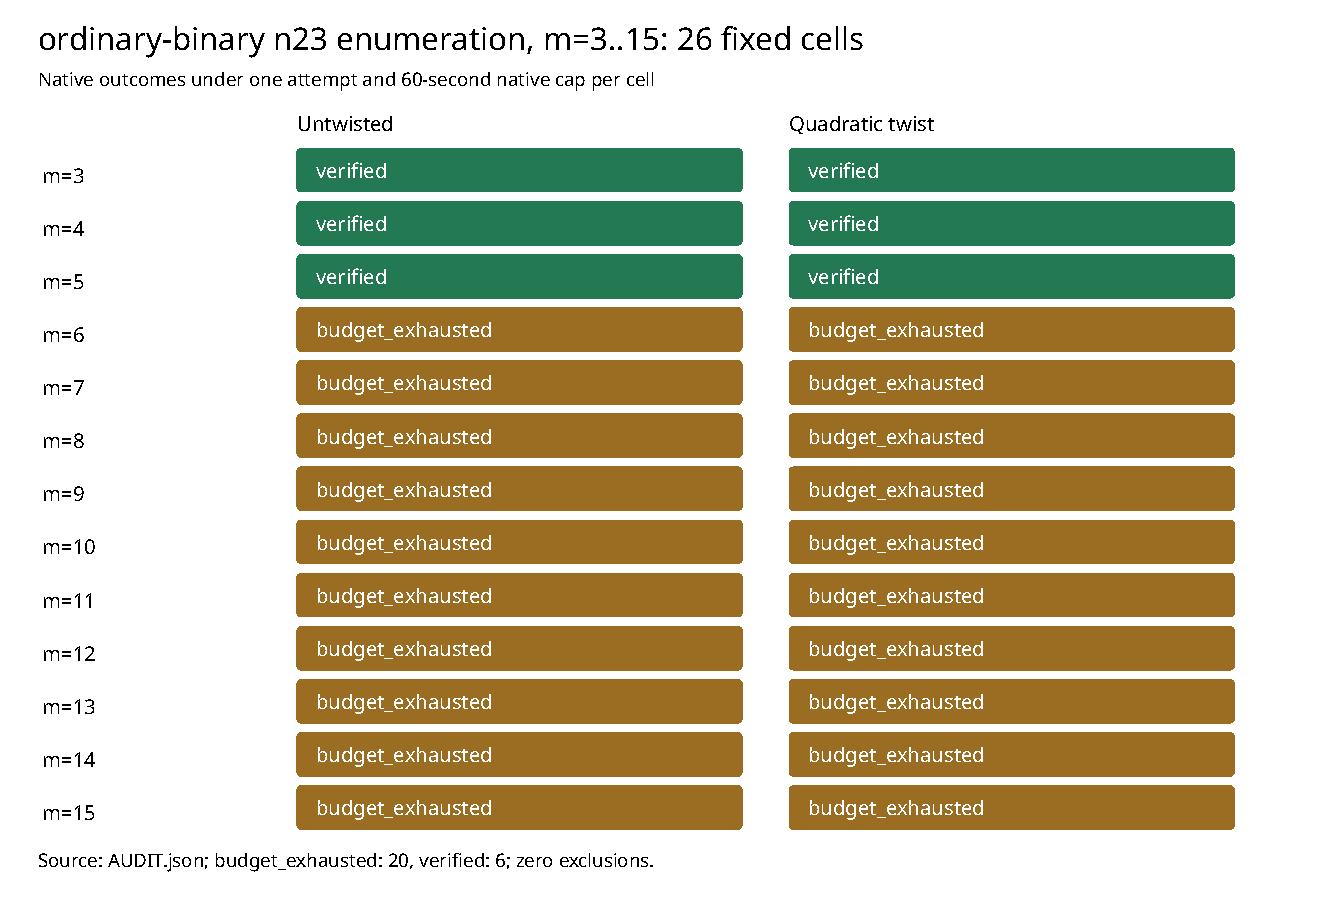
\includegraphics[width=0.92\linewidth]{outcomes.pdf}\end{center}

\subsection*{Exact evidence and measurement scope}
The pinned official export checker accepted 26 planned and attempted rows,
all completed with zero exclusions. Independent audit rehashed 26 archives
totalling 7,001,623 bytes and 832 native artifacts. It checked ordinary-binary
point-count/twist certificates, coefficient-field degree 23, and matched
public inputs across arities. At m3 each cell recorded 64 candidates and 84
group-add transitions, at m4 256 and 340, and at m5 1,024 and 1,364.

There are 104 retained phase telemetry records and zero eligible whole-worker
instruction labels. The fixed population supports exact method and custody
accounting, with no timing-effect comparison. See \texttt{report/run.md} for
hashes, receipts, and the distinct planted-positive control dependency.
\end{document}
